\documentclass{beamer}
%diuf beamer template
%example presentation: 
%%%%%%%%%%%%%%%%%%%%%%%%%%%%%
%%\documentclass{beamer}
%%%diuf beamer template
%example presentation: 
%%%%%%%%%%%%%%%%%%%%%%%%%%%%%
%%\documentclass{beamer}
%%%diuf beamer template
%example presentation: 
%%%%%%%%%%%%%%%%%%%%%%%%%%%%%
%%\documentclass{beamer}
%%\include{diuf}
%%\title{DIUF Beamer template}
%%\author{Tom Forrer}
%%\date[2009]{26.04.2009}
%%\institute{TNS}
%%\begin{document}
%%	\hskip-1cm\maketitle
%%\begin{frame}
%%	\frametitle{Outline}
%%	\tableofcontents
%%\end{frame}
%%\section{Introduction}
%%\subsection{Hello World}
%%\begin{frame}
%%	\frametitle{Hello World}
%%	\begin{itemize}
%%		\item Item
%%	\end{itemize}
%%	\begin{block}{Theorem}
%%			Test
%%	\end{block}
%%\end{frame}
%%\end{document}
%%%%%%%%%%%%%%%%%%%%%%%%%%%%%
\usepackage[latin1]{inputenc}

\setbeamercovered{dynamic} % shows items in white grey before active
%diuf green replaces standard blendedblue
\definecolor{beamer@blendedblue}{rgb}{0.0,0.6,0.439}
%diuf uses squares instead of triangles
\setbeamertemplate{items}[square]
%add indent and horizontal green bar to the frame titles
\setbeamertemplate{frametitle}
{
    \vskip-36pt %-8pt when documentclass is set with 10pt
	\ifbeamercolorempty[bg]{frametitle}{}{\nointerlineskip}
	\hspace*{0.1\textwidth}\color{beamer@blendedblue}\rule{1.1\textwidth}{10pt}\hspace*{-1.6cm}\vspace*{-5pt}{\color{white}\begin{tiny}\insertframenumber\,/\,\inserttotalframenumber\end{tiny}}\vspace*{10pt}
	\hspace*{0.1\textwidth}\usebeamerfont{frametitle}\color{beamer@blendedblue}\insertframetitle 
}
%add diuf logo on the footer section
\setbeamertemplate{sidebar left}
{ 
	\vfill 
	\rlap{\hskip0pt
	
\includegraphics[width=1.4\textwidth]{diuf.png} } %1.19
} 
%small tree on the upper left
\useoutertheme{tree}
%adjust left margin
\setbeamersize{text margin left=2.6cm}
%block environment
\setbeamertemplate{blocks}[rounded][shadow=true]
\setbeamercolor{block title}{bg = beamer@blendedblue, fg=white}

%%\title{DIUF Beamer template}
%%\author{Tom Forrer}
%%\date[2009]{26.04.2009}
%%\institute{TNS}
%%\begin{document}
%%	\hskip-1cm\maketitle
%%\begin{frame}
%%	\frametitle{Outline}
%%	\tableofcontents
%%\end{frame}
%%\section{Introduction}
%%\subsection{Hello World}
%%\begin{frame}
%%	\frametitle{Hello World}
%%	\begin{itemize}
%%		\item Item
%%	\end{itemize}
%%	\begin{block}{Theorem}
%%			Test
%%	\end{block}
%%\end{frame}
%%\end{document}
%%%%%%%%%%%%%%%%%%%%%%%%%%%%%
\usepackage[latin1]{inputenc}

\setbeamercovered{dynamic} % shows items in white grey before active
%diuf green replaces standard blendedblue
\definecolor{beamer@blendedblue}{rgb}{0.0,0.6,0.439}
%diuf uses squares instead of triangles
\setbeamertemplate{items}[square]
%add indent and horizontal green bar to the frame titles
\setbeamertemplate{frametitle}
{
    \vskip-36pt %-8pt when documentclass is set with 10pt
	\ifbeamercolorempty[bg]{frametitle}{}{\nointerlineskip}
	\hspace*{0.1\textwidth}\color{beamer@blendedblue}\rule{1.1\textwidth}{10pt}\hspace*{-1.6cm}\vspace*{-5pt}{\color{white}\begin{tiny}\insertframenumber\,/\,\inserttotalframenumber\end{tiny}}\vspace*{10pt}
	\hspace*{0.1\textwidth}\usebeamerfont{frametitle}\color{beamer@blendedblue}\insertframetitle 
}
%add diuf logo on the footer section
\setbeamertemplate{sidebar left}
{ 
	\vfill 
	\rlap{\hskip0pt
	
\includegraphics[width=1.4\textwidth]{diuf.png} } %1.19
} 
%small tree on the upper left
\useoutertheme{tree}
%adjust left margin
\setbeamersize{text margin left=2.6cm}
%block environment
\setbeamertemplate{blocks}[rounded][shadow=true]
\setbeamercolor{block title}{bg = beamer@blendedblue, fg=white}

%%\title{DIUF Beamer template}
%%\author{Tom Forrer}
%%\date[2009]{26.04.2009}
%%\institute{TNS}
%%\begin{document}
%%	\hskip-1cm\maketitle
%%\begin{frame}
%%	\frametitle{Outline}
%%	\tableofcontents
%%\end{frame}
%%\section{Introduction}
%%\subsection{Hello World}
%%\begin{frame}
%%	\frametitle{Hello World}
%%	\begin{itemize}
%%		\item Item
%%	\end{itemize}
%%	\begin{block}{Theorem}
%%			Test
%%	\end{block}
%%\end{frame}
%%\end{document}
%%%%%%%%%%%%%%%%%%%%%%%%%%%%%
\usepackage[latin1]{inputenc}

\setbeamercovered{dynamic} % shows items in white grey before active
%diuf green replaces standard blendedblue
\definecolor{beamer@blendedblue}{rgb}{0.0,0.6,0.439}
%diuf uses squares instead of triangles
\setbeamertemplate{items}[square]
%add indent and horizontal green bar to the frame titles
\setbeamertemplate{frametitle}
{
    \vskip-36pt %-8pt when documentclass is set with 10pt
	\ifbeamercolorempty[bg]{frametitle}{}{\nointerlineskip}
	\hspace*{0.1\textwidth}\color{beamer@blendedblue}\rule{1.1\textwidth}{10pt}\hspace*{-1.6cm}\vspace*{-5pt}{\color{white}\begin{tiny}\insertframenumber\,/\,\inserttotalframenumber\end{tiny}}\vspace*{10pt}
	\hspace*{0.1\textwidth}\usebeamerfont{frametitle}\color{beamer@blendedblue}\insertframetitle 
}
%add diuf logo on the footer section
\setbeamertemplate{sidebar left}
{ 
	\vfill 
	\rlap{\hskip0pt
	
\includegraphics[width=1.4\textwidth]{diuf.png} } %1.19
} 
%small tree on the upper left
\useoutertheme{tree}
%adjust left margin
\setbeamersize{text margin left=2.6cm}
%block environment
\setbeamertemplate{blocks}[rounded][shadow=true]
\setbeamercolor{block title}{bg = beamer@blendedblue, fg=white}

\usepackage{tabularx}
\usepackage{multirow}
\usepackage{dcolumn}
%% Kommandos fuer Tabellen. Entnommen aus The LateX Companion, tabsatz.ps und diversen Dokus:

%%% ---| Farben fuer Tabellen |-------------------
\IfPackageLoaded{xcolor}{
   \colorlet{tablesubheadcolor}{gray!30}
   \colorlet{tableheadcolor}{gray!25}
   \colorlet{tableblackheadcolor}{black!100}
   \colorlet{tablerowcolor}{gray!10.0}
}
%%% ---------------------------------------------


%%% -| Neue Spaltendefinitionen 'columntypes' |--
%
% Belegte Spaltentypen:
% l - links
% c - zentriert
% r - rechts
% p,m,b  - oben, mittig, unten
% X - tabularx Auto-Spalte

% um Tabellenspalten mit Flattersatz zu setzen, muss \\ vor
% (z.B.) \raggedright geschuetzt werden:
\newcommand{\PreserveBackslash}[1]{\let\temp=\\#1\let\\=\temp}


% Spalten mit Flattersatz und definierte Breite:
% m{} -> mittig
% p{} -> oben
% b{} -> unten
%
% Linksbuendig:
\newcolumntype{v}[1]{>{\PreserveBackslash\RaggedRight\hspace{0pt}}p{#1}}
\newcolumntype{M}[1]{>{\PreserveBackslash\RaggedRight\hspace{0pt}}m{#1}}
% % Rechtsbuendig :
% \newcolumntype{R}[1]{>{\PreserveBackslash\RaggedLeft\hspace{0pt}}m{#1}}
% \newcolumntype{S}[1]{>{\PreserveBackslash\RaggedLeft\hspace{0pt}}p{#1}}
% % Zentriert :
% \newcolumntype{Z}[1]{>{\PreserveBackslash\Centering\hspace{0pt}}m{#1}}
% \newcolumntype{A}[1]{>{\PreserveBackslash\Centering\hspace{0pt}}p{#1}}

\newcolumntype{Y}{>{\PreserveBackslash\RaggedLeft\hspace{0pt}}X}
%%% Spalten fuer Mathematik
%
% serifenlose Matheschrift
\newcolumntype{s}[1]{%
	>{\DC@{.}{,}{#1}\mathsf\bgroup}l%
	<{\egroup\DV@end}%
}

% Tabellenspaltentyp fuer den Kopf: (Farbe + Ausrichtung)
\newcolumntype{H}[1]{>{\columncolor{tableheadcolor}}l}

% aequivalent aus typokurz (fett+grau+links)
% \newcolumntype{H}{>{\fontseries{b}\selectfont%
%     \columncolor[gray]{.8}[6pt][0pt]}l}
%%% --------------------------------------------


%%% ---|Listen in Tabellen |--------------------
\newcommand{\removeindentation}{%
	\leftmargini=\labelsep%
	\advance\leftmargini by \labelsep%
}
%
\makeatletter
\newcommand\tableitemize{
	\@minipagetrue%
	\removeindentation
}
\makeatother
%%% --------------------------------------------

%%% ---|Layout der Tabellen |-------------------

% Neue Umgebung fuer Tabellen:

\newenvironment{Tabelle}[2][c]{%
  \tablestylecommon
  \begin{longtable}[#1]{#2}
  }
  {\end{longtable}%
  \tablerestoresettings
}


% Groesse der Schrift in Tabellen
\newcommand{\tablefontsize}{ \footnotesize}
\newcommand{\tableheadfontsize}{\footnotesize}

% Layout der Tabelle: Ausrichtung, Schrift, Zeilenabstand
\newcommand\tablestylecommon{%
  \renewcommand{\arraystretch}{1.4} % Groessere Abstaende zwischen Zeilen
  \normalfont\normalsize            %
  \sffamily\tablefontsize           % Serifenlose und kleine Schrift
  \centering%                       % Tabelle zentrieren
}

\newcommand{\tablestyle}{
	\tablestylecommon
	%\tablealtcolored
}

% Ruecksetzten der Aenderungen
\newcommand\tablerestoresettings{%
  \renewcommand{\arraystretch}{1}% Abstaende wieder zuruecksetzen
  \normalsize\rmfamily % Schrift wieder zuruecksetzen
}

% Tabellenkopf: Serifenlos+fett+schraeg+Schriftfarbe
\newcommand\tablehead{%
  \tableheadfontsize%
  \sffamily\bfseries%
  %\slshape
  %\color{white}
}

\newcommand\tablesubheadfont{%
  \tableheadfontsize%
  \sffamily\bfseries%
  \slshape
  %\color{white}
}


\newcommand\tableheadcolor{%
	%\rowcolor{tablesubheadcolor}
	%\rowcolor{tableblackheadcolor}
	\rowcolor{tableheadcolor}%
}

\newcommand\tablesubheadcolor{%
	\rowcolor{tablesubheadcolor}
	%\rowcolor{tableblackheadcolor}
}


\newcommand{\tableend}{\arrayrulecolor{black}\hline}

% Tabellenkopf (1=Spaltentyp, 2=Text)
% \newcommand{\tablehead}[2]{
%   \multicolumn{1}{#1@{}}{%
%     \raisebox{.1mm}{% Ausrichtung der Beschriftung
%       #2%
%     }\rule{0pt}{4mm}}% unsichtbare Linie, die die Kopfzeile hoeher macht
% }


\newcommand{\tablesubhead}[2]{%
  \multicolumn{#1}{>{\columncolor{tablesubheadcolor}}l}{\tablesubheadfont #2}%
}

% Tabellenbody (=Inhalt)
\newcommand\tablebody{%
\tablefontsize\sffamily\upshape%
}

\newcommand\tableheadshaded{%
	\rowcolor{tableheadcolor}%
}
\newcommand\tablealtcolored{%
	\rowcolors{1}{tablerowcolor}{white!100}%
}
%%% --------------------------------------------

\newlength{\mylen}
\newlength{\adjusthspace}

\newenvironment{tabularc}[2]
{%
	\setlength\mylen{#2/(#1)-\tabcolsep*2-\arrayrulewidth*(#1+1)/(#1)}%
	%\setlength{\adjusthspace}{((#2-1)/2)*\linewidth}
	%\par\noindent
	%\hspace*{-\the\adjusthspace}
	\begin{tabular}%{#2}%
		{*{#1}{v{\the\mylen}}}%
}
{\end{tabular}\par}


\title{Ergonomic Gestures Recognition\\ 
\includegraphics[scale=0.2]{images/egr}}
\author{Tom Forrer}
\date[2011]{27.01.2011}
\institute{DIVA}

\begin{document}

	\hskip-1cm\maketitle

	\begin{frame}
		\frametitle{Outline}
		\vspace*{-0.4cm}
		\tableofcontents
	\end{frame}
	
	\section{Introduction}
%	\subsection{Context}
%	\begin{frame}
%		\frametitle{Context}
%		\begin{itemize}
%			\item 
%		\end{itemize}
%	\end{frame}
	
	\subsection{Ergonomic gestures}
	\begin{frame}
		\frametitle{Ergonomic gestures}
		Gestures for controlling an application that have:
		\begin{itemize}
			\item limited action space
			\item precision
			\item wrist or arm support
			\item comfort
		\end{itemize}
	\end{frame}
	\subsection{Goals}
	\begin{frame}
		\frametitle{Goals}
		\begin{itemize}
			\item Recognize spatial and temporal aspects of ergonomic gestures
			\item Build an architecture capable of real-time gesture recognition
			\item Implement a demonstration program using this architecture
		\end{itemize}
	\end{frame}
	\section{State of the art}
	\begin{frame}
		\frametitle{State of the art: tracking}
		\begin{figure}
			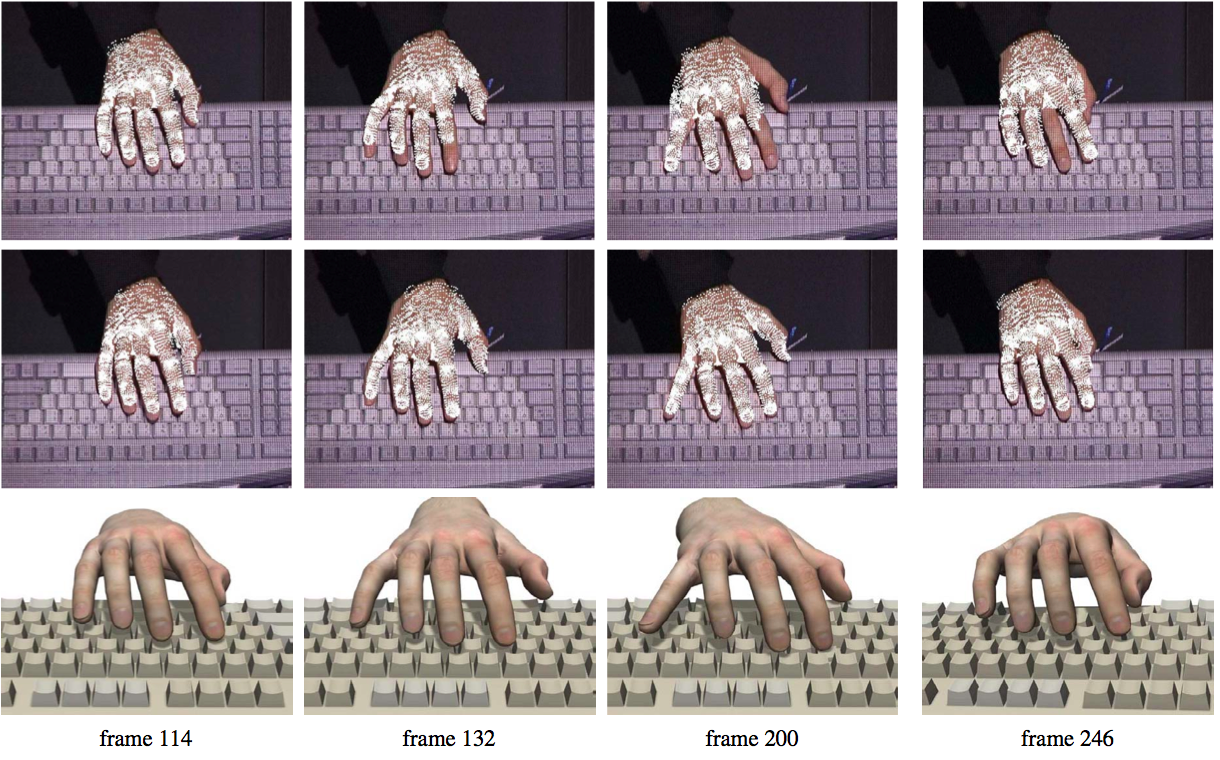
\includegraphics[scale=0.2]{images/gool} 
			\caption{Bray, Koller-Meier, Van Gool: SPF particle filter, 3D hand-model (15 DOF)}
		\end{figure}
	\end{frame}
	\begin{frame}
		\frametitle{State of the art: tracking}
		\begin{figure}
			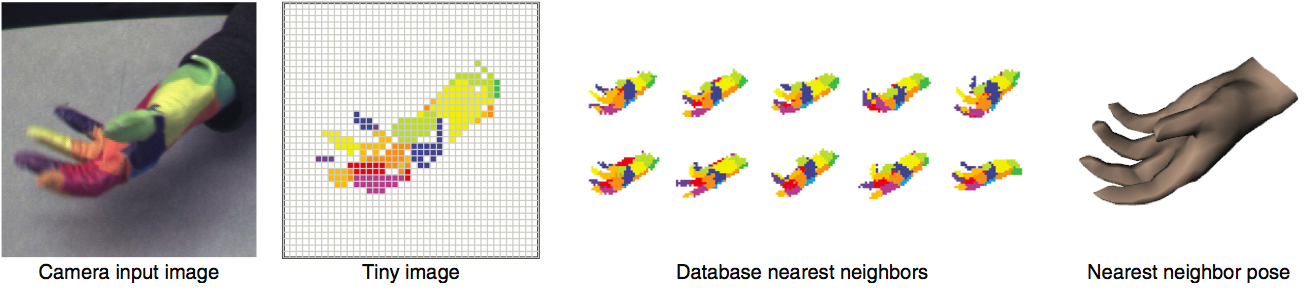
\includegraphics[scale=0.2]{images/wang} 
			\caption{Wang, Popovic: Real-time hand tracking with color glove }
		\end{figure}
	\end{frame}
	\begin{frame}
		\frametitle{State of the art: recognition}
		\begin{figure}
			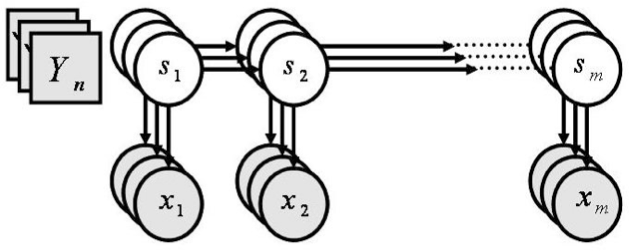
\includegraphics[scale=0.15]{images/seminar/hmm} 
			\caption{Hidden Markov Model}
		\end{figure}
		
		\begin{figure}
			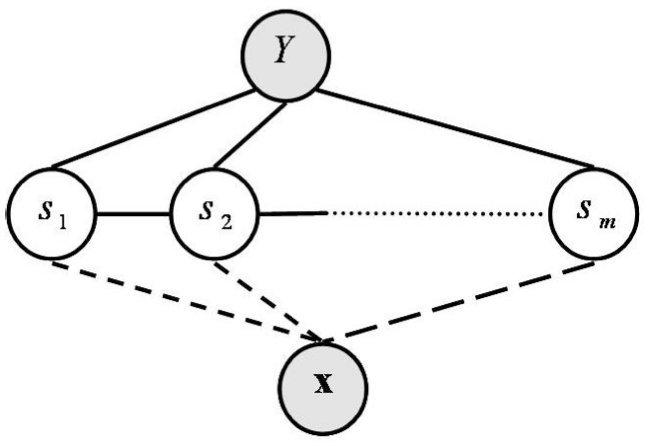
\includegraphics[scale=0.15]{images/seminar/hcrf} 
			\caption{Sy Bor Wang et al: Hidden conditional random fields}
		\end{figure}
	\end{frame}
	\section{Hardware \& Software}
	\subsection*{Hardware}
	\begin{frame}
		\frametitle{Camera}
		\begin{figure}
			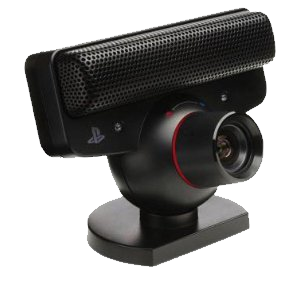
\includegraphics[scale=0.3]{images/ps3eye} 
			\caption{Playstation 3 Eye Camera}
		\end{figure}
		\vspace*{-0.5cm}
		\begin{itemize}
			\item Resolution: 640$\times$480
			\item Frame rate: 60 fps $@$ 640$\times$480, 120 fps $@$ 320$\times$240
			\item Color and image fidelity
			\item Price
		\end{itemize}
	\end{frame}
	\begin{frame}
		\frametitle{Glove}
		\begin{figure}
			\hspace*{-1cm}
			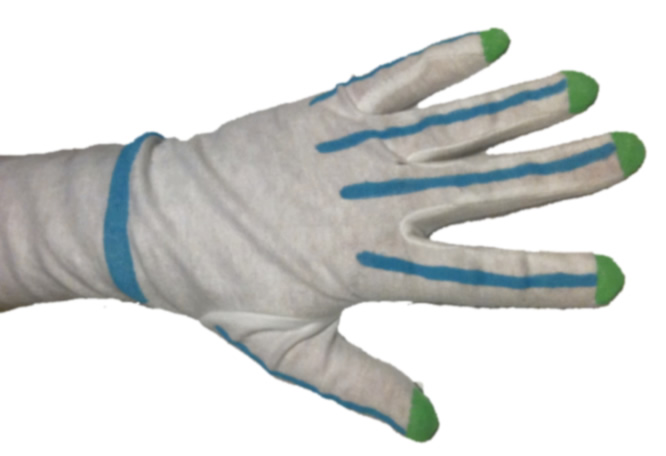
\includegraphics[width=0.33\textwidth]{images/glovev1} \hspace*{0.2cm}
			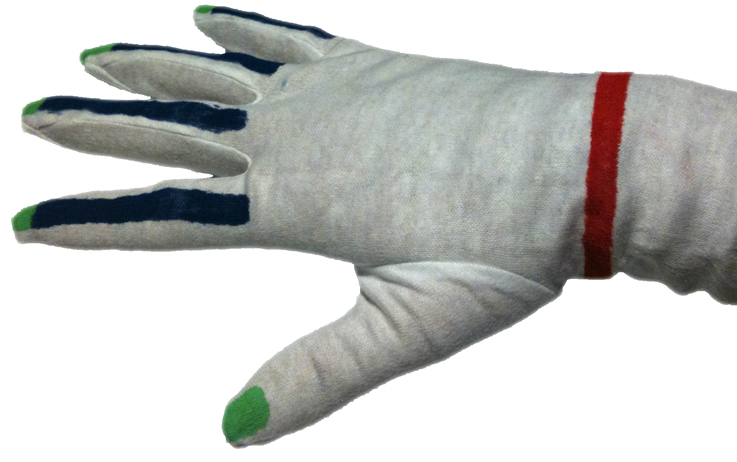
\includegraphics[width=0.33\textwidth]{images/glovev2} \hspace*{0.2cm}
			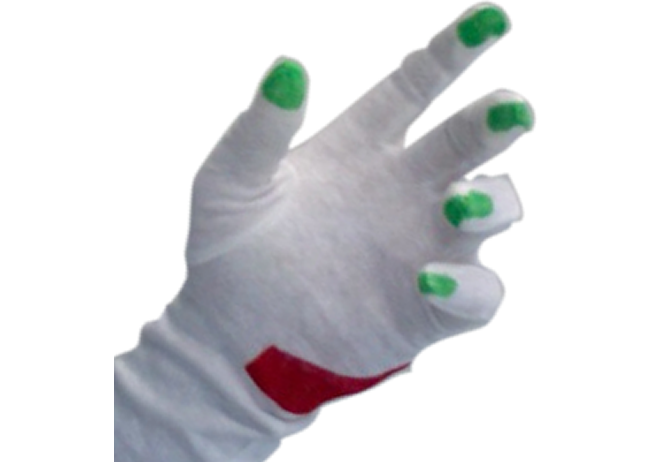
\includegraphics[width=0.33\textwidth]{images/glovev3} 
			\caption{Textile glove with color markers}
		\end{figure}
		\vspace*{-0.5cm}
		\begin{itemize}	
			\item Color-marked finger positions (green)
			\item Color-marked wrist position (red)
			\item Easy to put on and off
		\end{itemize}
	\end{frame}
	\subsection*{Setup}
	\begin{frame}
		\frametitle{Setup}
		\begin{figure}
			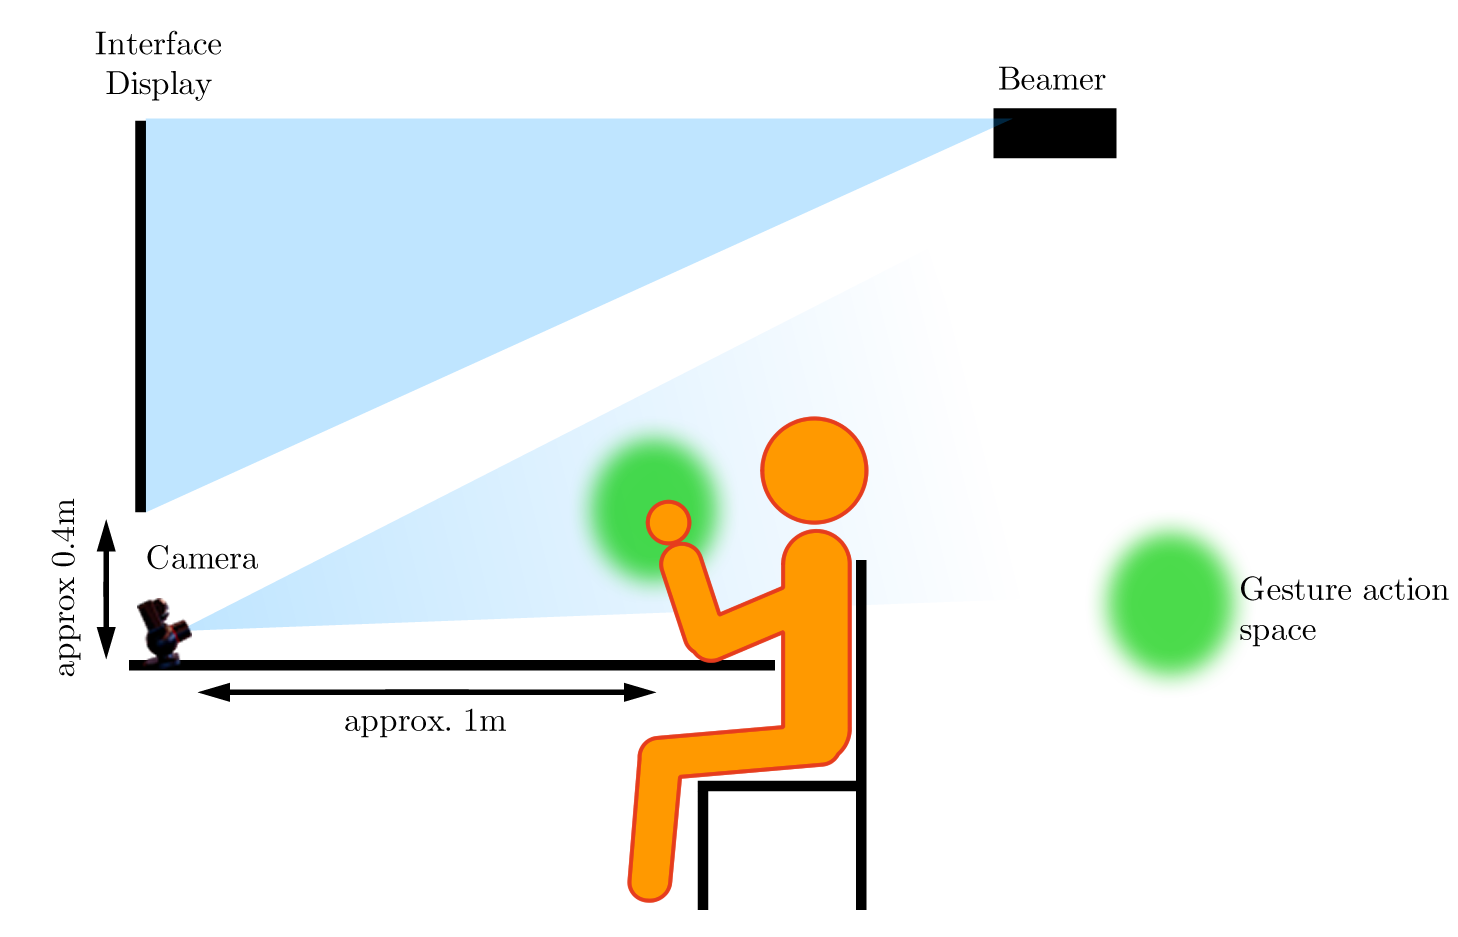
\includegraphics[scale=0.3]{images/setup} 
			\caption{Environmental setup}
		\end{figure}
	\end{frame}
	
	\subsection*{Software}
	\begin{frame}
		\frametitle{Software}
		\begin{itemize}
			\item Visual Studio 2008: C++
			\item OpenCV 2.0
			\item dlib C++ ML
			\item Qt 4.7
			\item libconfig
		\end{itemize}
	\end{frame}
	\section{Gestures}
	\begin{frame}
		\frametitle{Chosen gestures}
		\begin{figure}
			\hspace*{-2cm}
			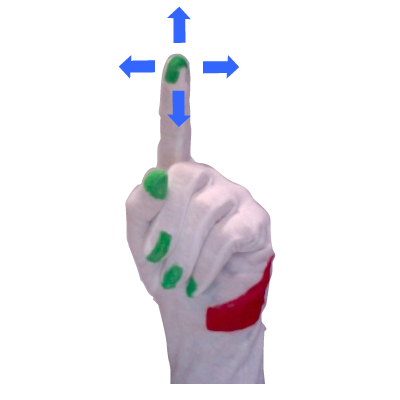
\includegraphics[width=0.3\textwidth]{images/gesture_pointing} \hspace*{0.1cm}
			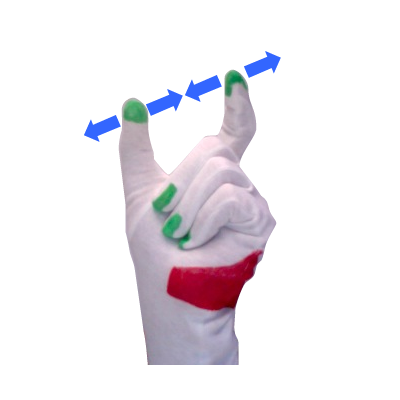
\includegraphics[width=0.3\textwidth]{images/gesture_zooming} \hspace*{0.1cm}
			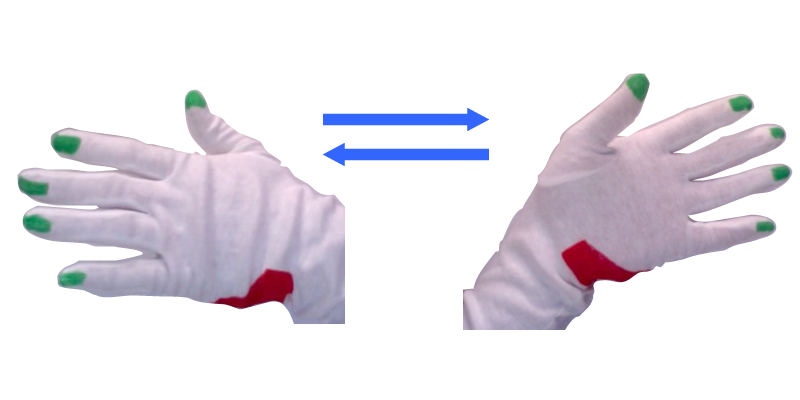
\includegraphics[width=0.6\textwidth]{images/gesture_swiping} 
			\caption{Pointing, zooming and horizontal swiping gesture}
		\end{figure}
	\end{frame}
	\section{Design and architecture}
	\begin{frame}
		\frametitle{Architecture}
		\begin{figure}
			\hspace*{-2cm}
			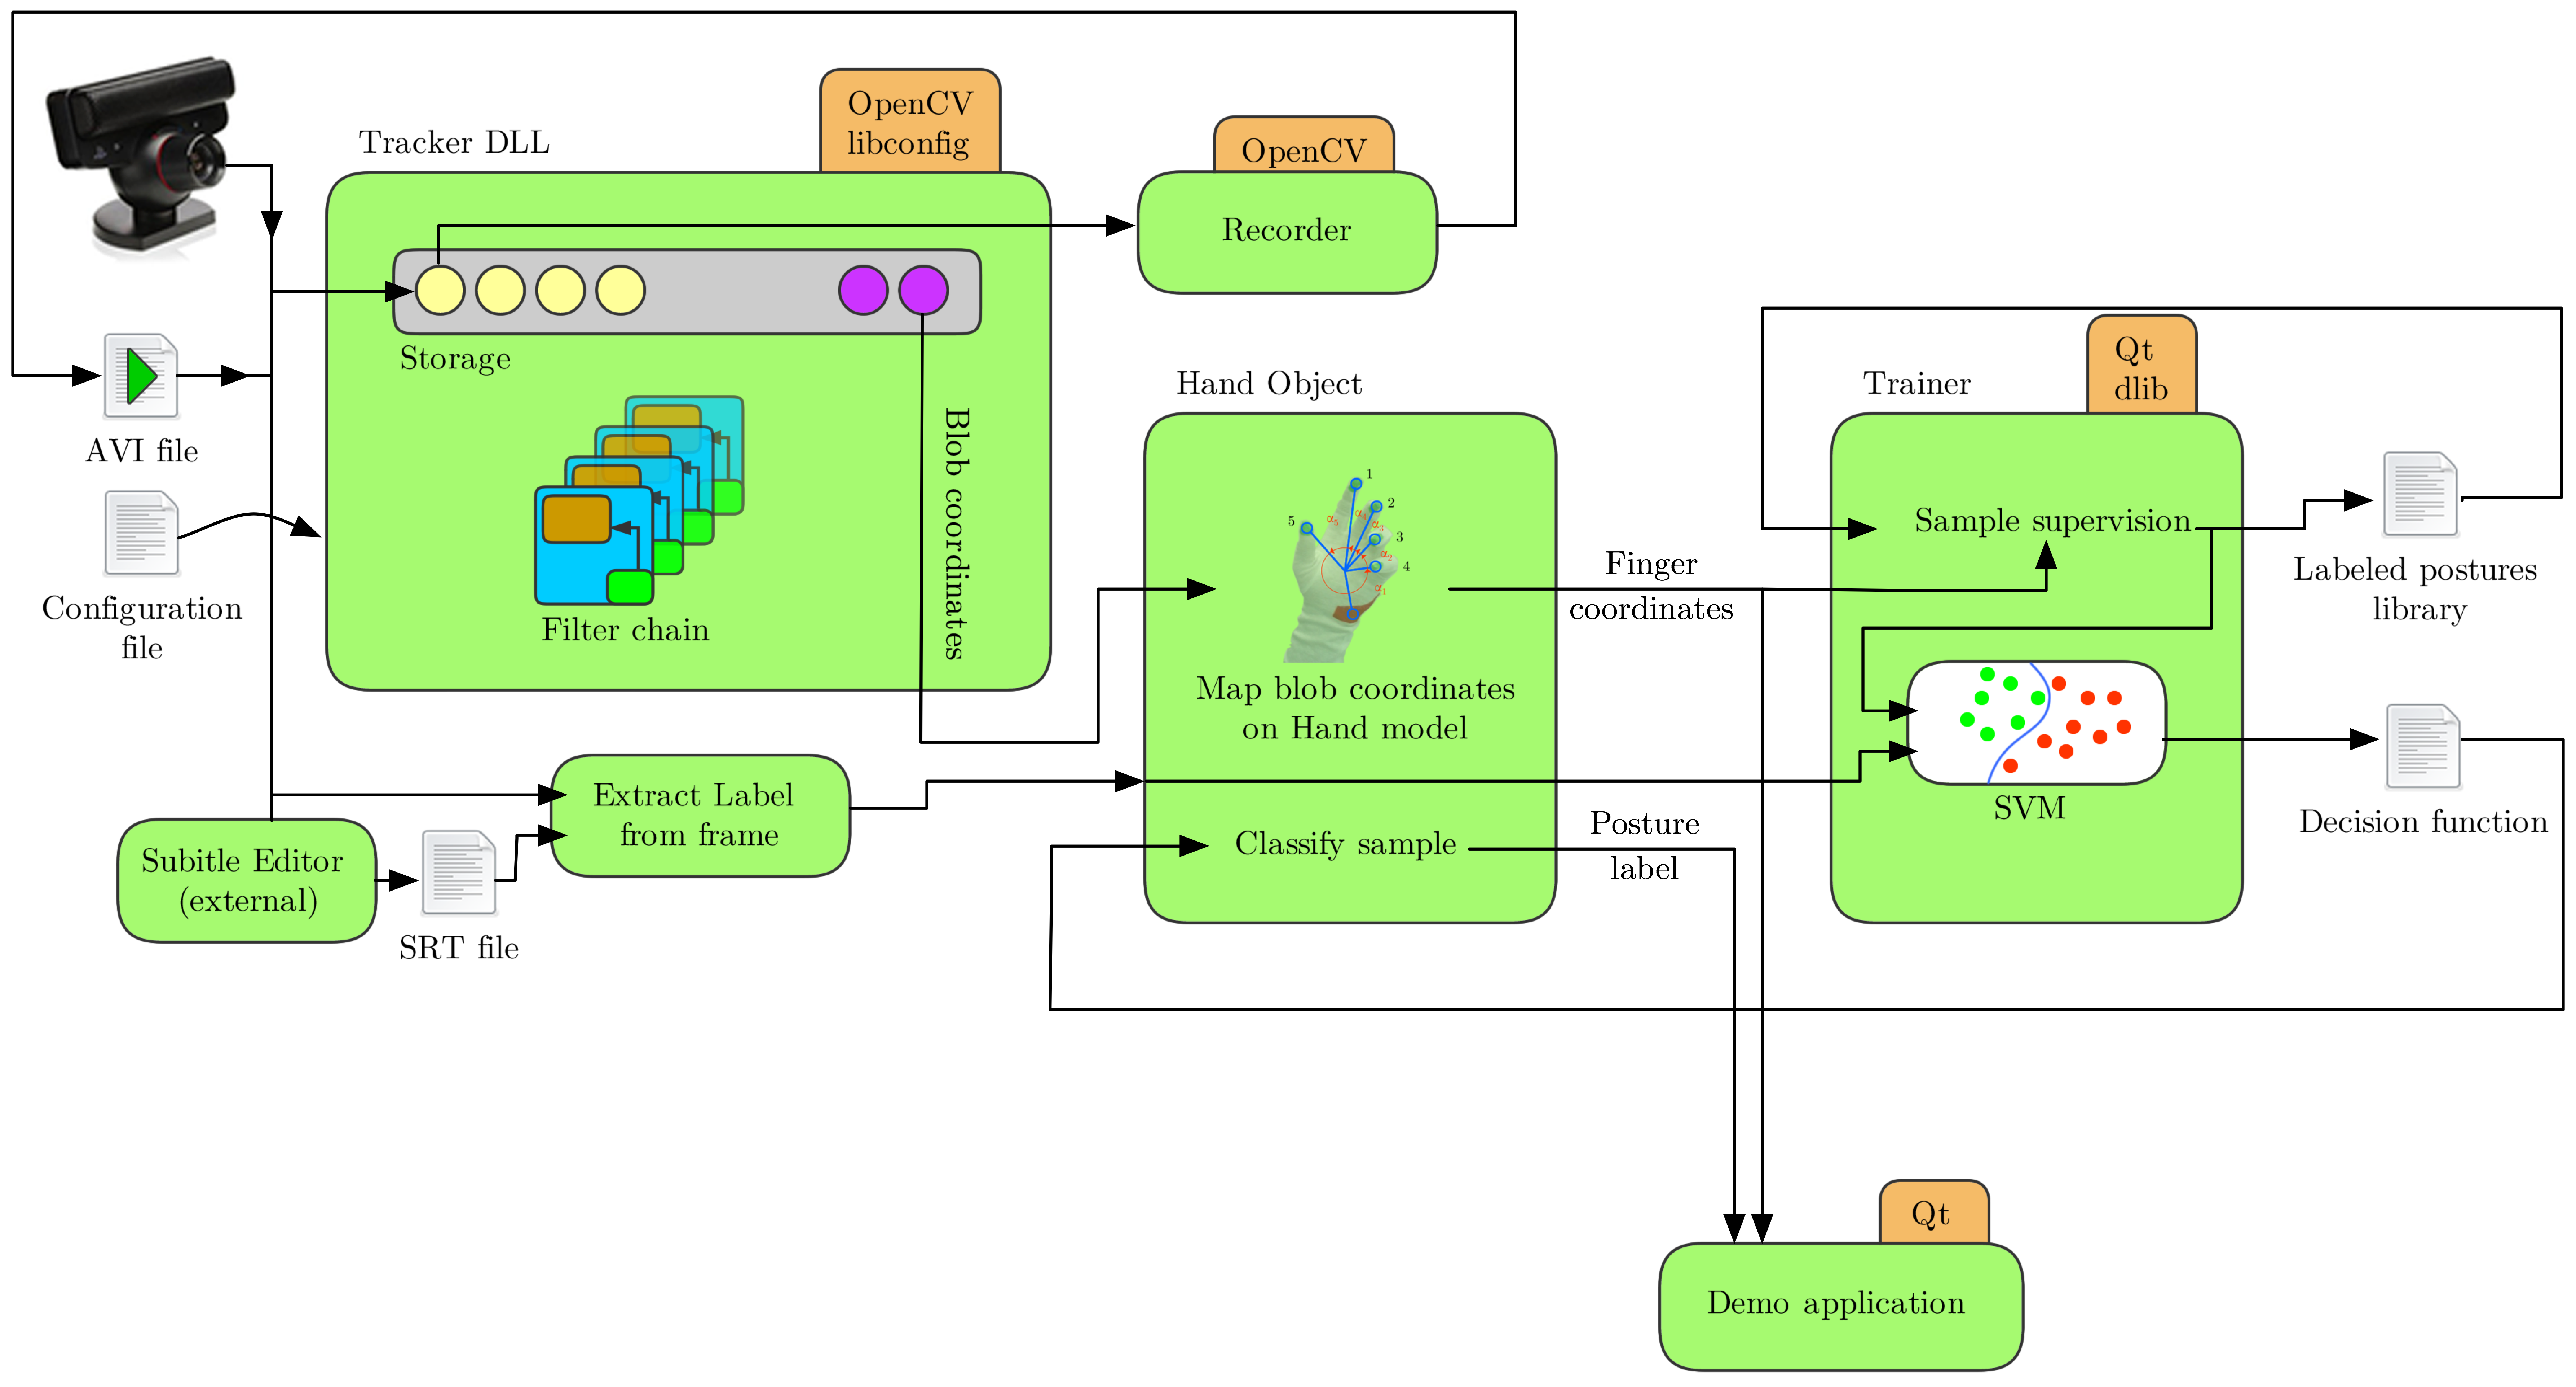
\includegraphics[width=1.3\textwidth]{images/arch} 
			%\caption{Architecture}
		\end{figure}
	\end{frame}
	\subsection{Tracker}
	\begin{frame}
		\frametitle{Tracker configuration}
		\begin{itemize}
			\item reconfigurable filter arrangement
			\item on-line parameter adjustement
			\item optimized for speed
			\item extendable image processing operations list: Lab Thresholding, RGB Thresholding, Binary Thresholding, Erosion, Dilation, Smooth, Blob detection, FAST corner detection, Add
		\end{itemize}
	\end{frame}
	\begin{frame}
		\frametitle{Filter chain}
		\begin{figure}
			\hspace*{-2cm}
			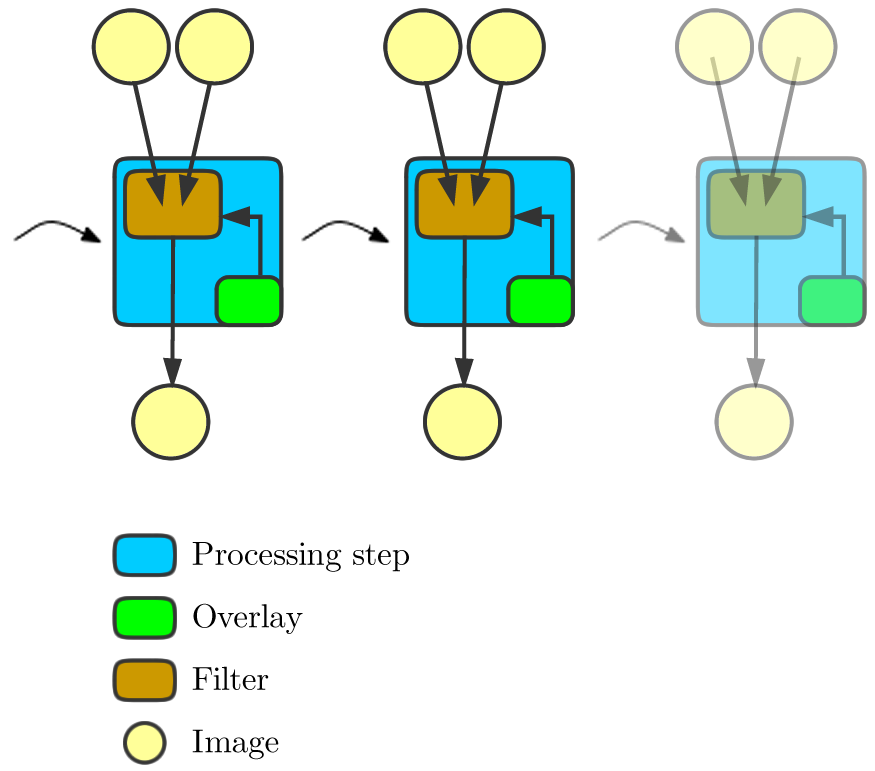
\includegraphics[width=0.7\textwidth]{images/steps_general} 
			\caption{Chain of reconfigurable processing elements}
		\end{figure}
	\end{frame}
	\begin{frame}
		\frametitle{Filter chain}
		\begin{figure}
			\hspace*{-2cm}
			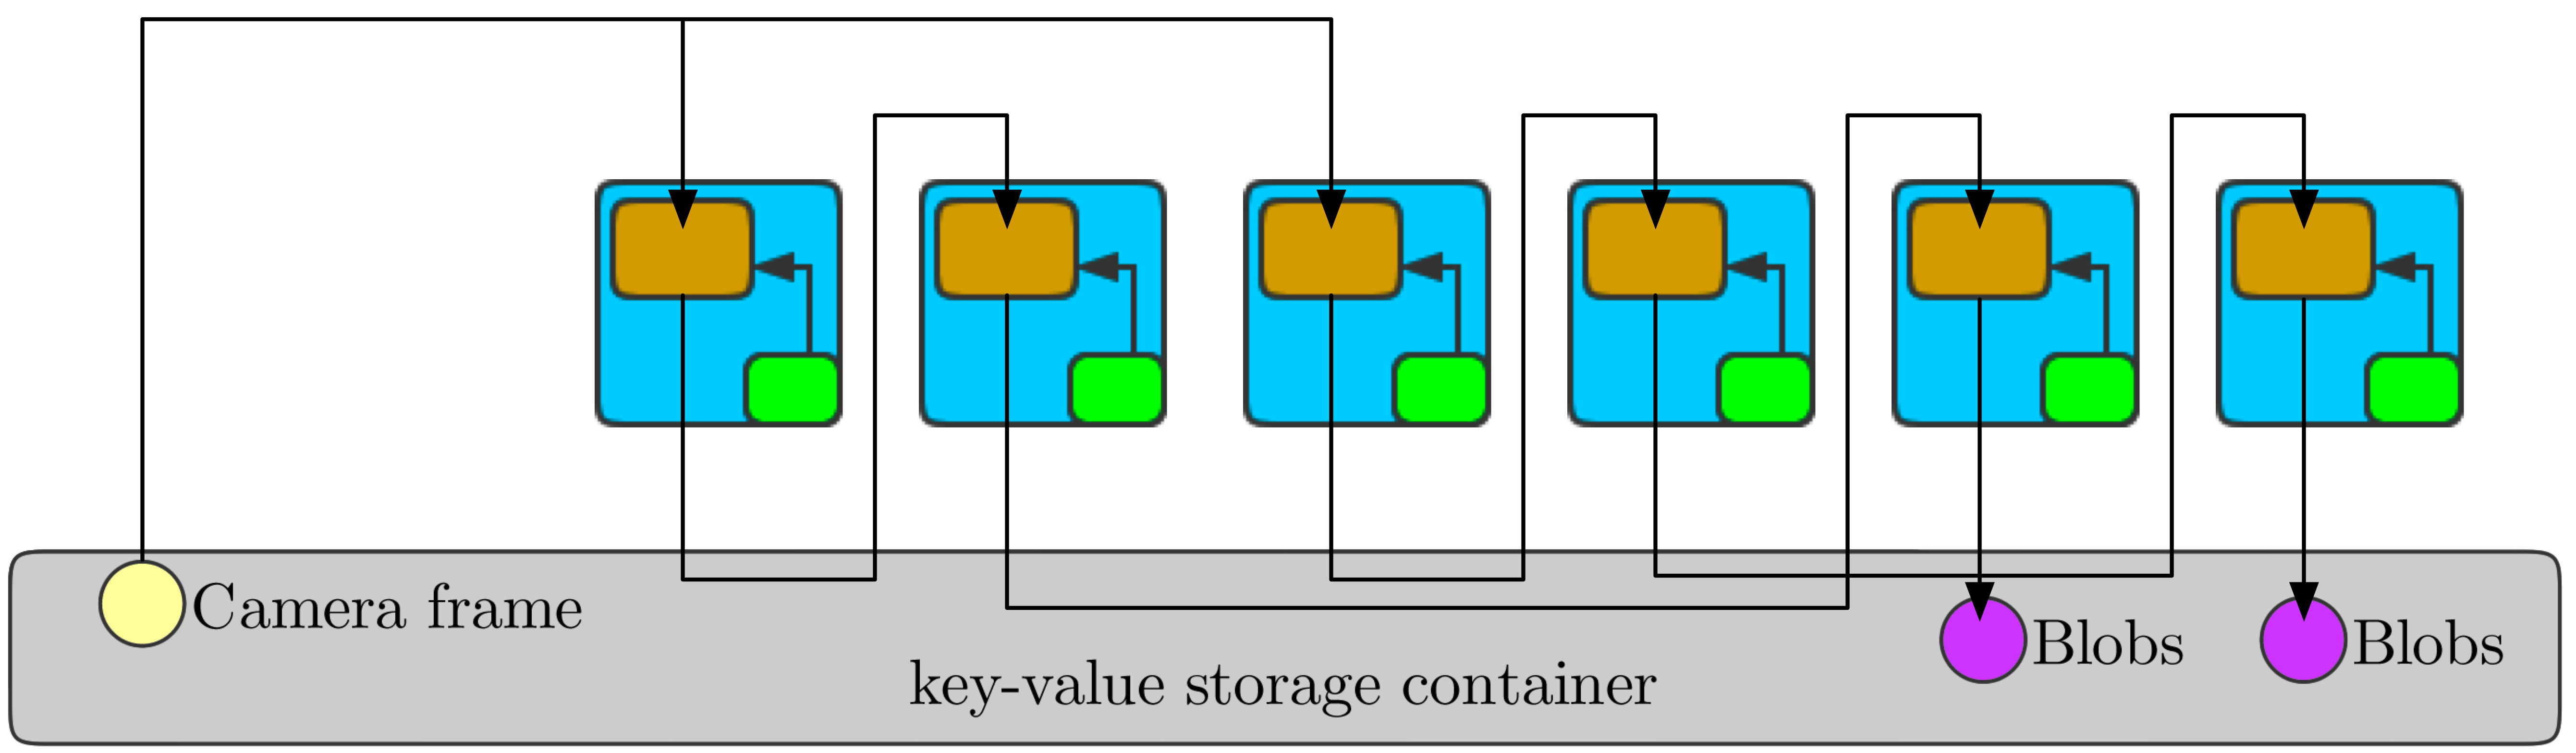
\includegraphics[width=1.3\textwidth]{images/steps_egr} 
			\caption{Chain of reconfigurable processing elements}
		\end{figure}
	\end{frame}
	\begin{frame}
		\frametitle{Filter chain}
		\begin{figure}
		\hspace*{-2cm}
			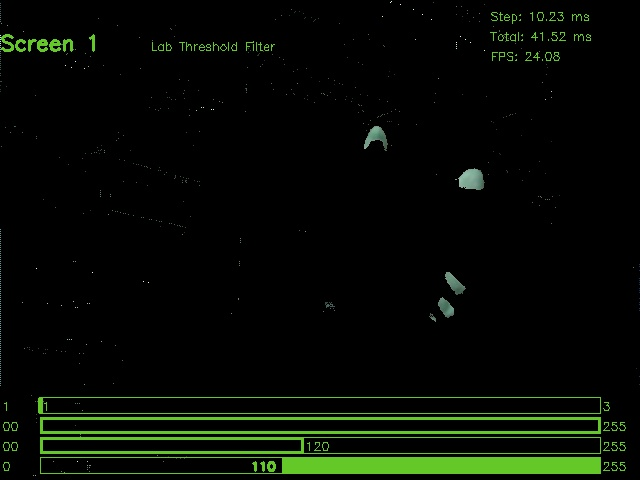
\includegraphics[width=0.25\textwidth]{images/lab_green} \hspace{0.2cm}
		    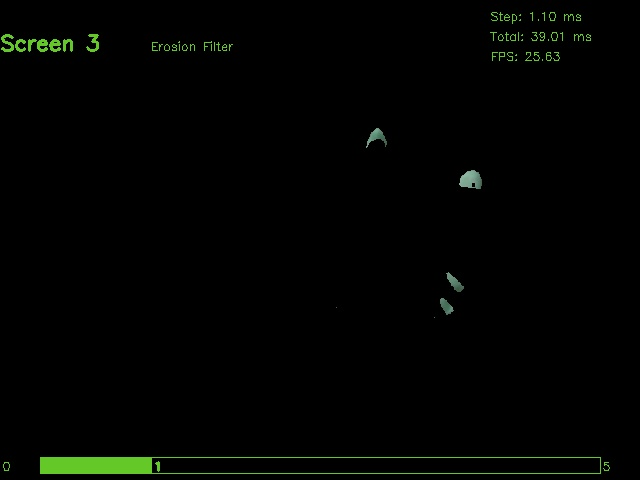
\includegraphics[width=0.25\textwidth]{images/erosion_green} \hspace{0.2cm}	
			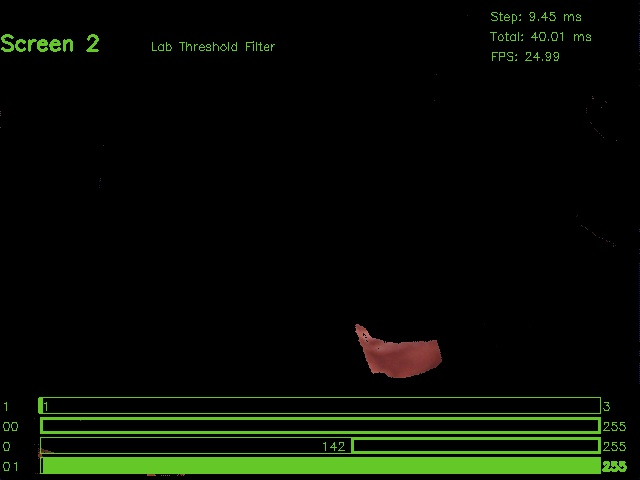
\includegraphics[width=0.25\textwidth]{images/lab_red} \hspace{0.2cm}
			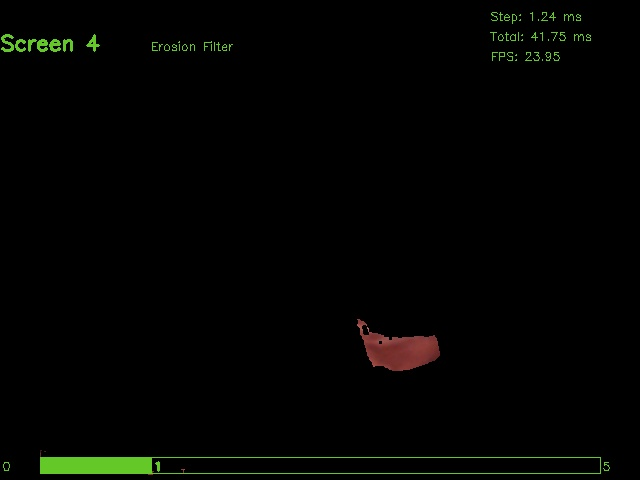
\includegraphics[width=0.25\textwidth]{images/erosion_red} \vspace*{0.5cm}\\
		\hspace*{-2cm}
			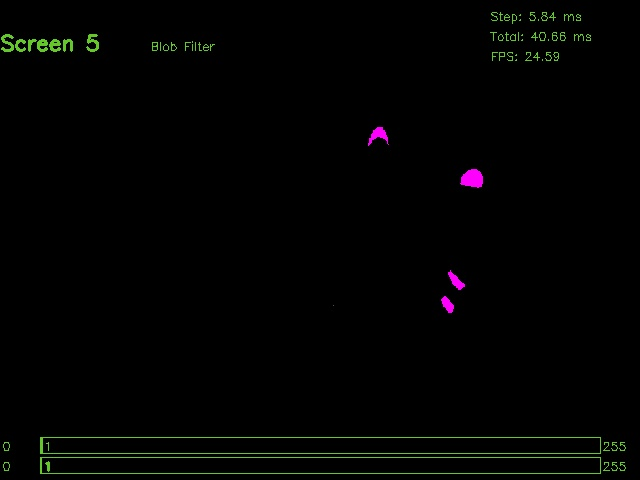
\includegraphics[width=0.25\textwidth]{images/blob_green} \hspace{0.2cm}
			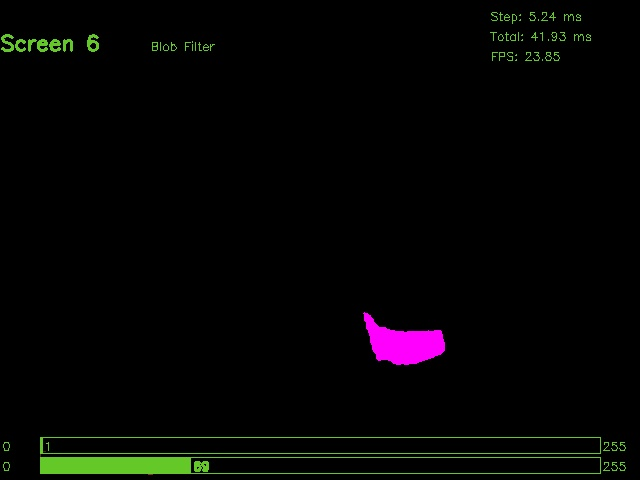
\includegraphics[width=0.25\textwidth]{images/blob_red} \hspace{0.2cm}
			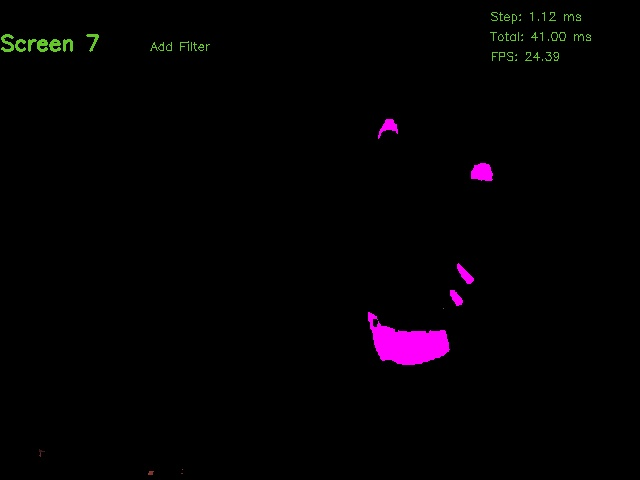
\includegraphics[width=0.25\textwidth]{images/add} \hspace{0.2cm}
			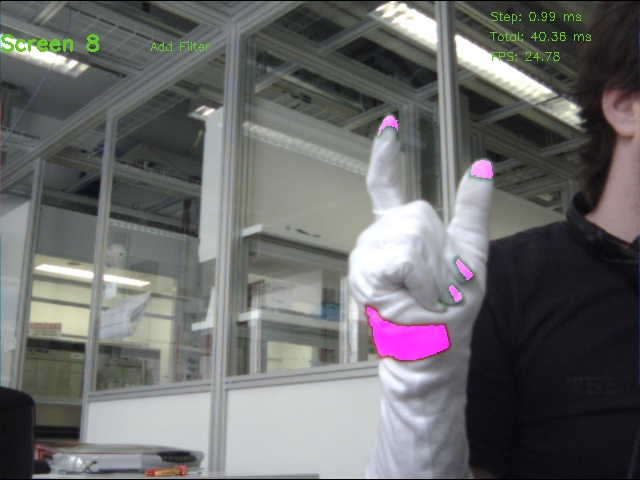
\includegraphics[width=0.25\textwidth]{images/overlay} 
		\caption{Resulting images from tracker with filter chain}
	
		\end{figure}
	\end{frame}
	\subsection{Model}
	\begin{frame}
		\frametitle{Hand model}
		\begin{itemize}
			\item Five fingers
			\item One wrist
			\item Fingers not crossed
			\item Angle
			\item Finger and wrist velocity
		\end{itemize}
	\end{frame}
	\begin{frame}
		\frametitle{Mapping}
		\begin{figure}
			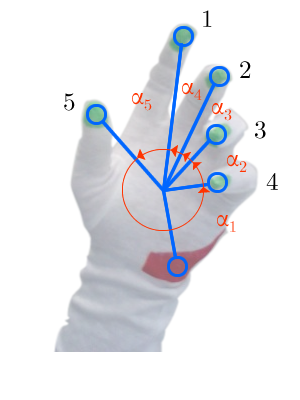
\includegraphics[height=0.7\textheight]{images/hand-model} 
			\caption{Hand-model mapping}
		\end{figure}
	\end{frame}
	\subsection{Training \& classification}
	\begin{frame}
		\frametitle{Sample collection}
		\begin{itemize}
			\item Record video of gestures with glove while respecting setup constraints
			\item Annotate postures with subtitle editor
			\item Collect labeled postures through tracker, hand model and subtitle file
			\item 55 seconds, 23 gestures, 23 FPS, 1251 postures
		\end{itemize}
	\end{frame}
	\begin{frame}
		\frametitle{Sample supervision}
		\begin{figure}
			\hspace*{-2cm}
			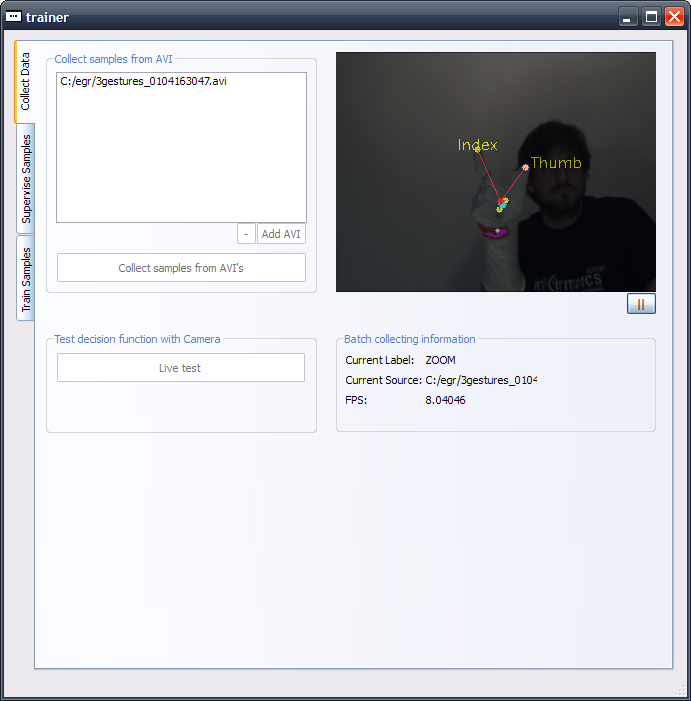
\includegraphics[height=0.65\textheight]{images/collect-samples} \hspace*{0.5cm}
			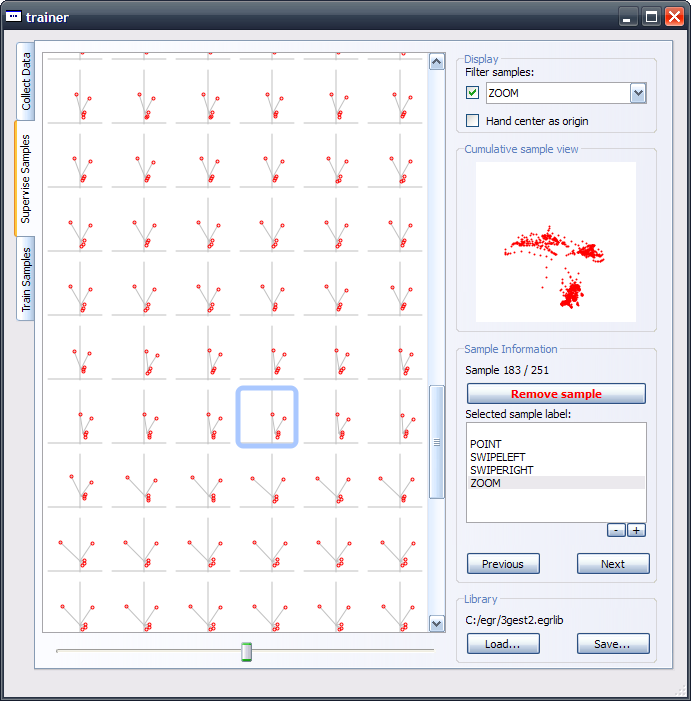
\includegraphics[height=0.65\textheight]{images/sample-supervision} 
			\caption{Sample collection and supervision}
		\end{figure}
	\end{frame}
	\begin{frame}
		\frametitle{Sample supervision}
		\begin{figure}
			\hspace*{-2cm}
			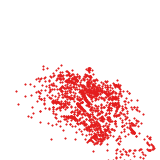
\includegraphics[width=0.2\textwidth]{images/allsamples-empty} \hspace*{0.2cm}
			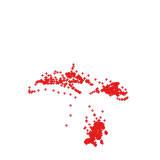
\includegraphics[width=0.2\textwidth]{images/allsamples-zoom} \hspace*{0.2cm}
			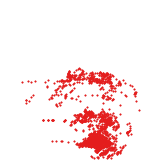
\includegraphics[width=0.2\textwidth]{images/allsamples-point} \hspace*{0.2cm}
			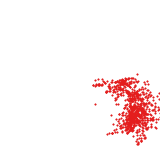
\includegraphics[width=0.2\textwidth]{images/allsamples-right} \hspace*{0.2cm}
			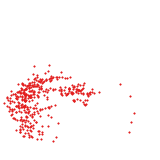
\includegraphics[width=0.2\textwidth]{images/allsamples-left}
			\caption{Sample collection and supervision}
		\end{figure}
		\begin{figure}
			\hspace*{-2cm}
			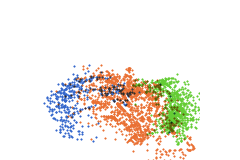
\includegraphics[width=0.33\textwidth]{images/allsamples-left-nothing-right} \hspace*{0.2cm}
			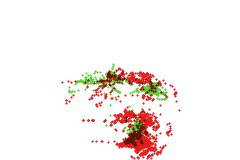
\includegraphics[width=0.33\textwidth]{images/allsamples-point-zoom} \hspace*{0.2cm}
			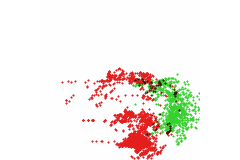
\includegraphics[width=0.33\textwidth]{images/allsamples-point-right} 
			\caption{Sample collection and supervision}
		\end{figure}
		
	\end{frame}
	\begin{frame}
		\frametitle{Posture training}
		Train a one-vs-one multiclass $\nu$-Support Vector Machine with polynomial kernels
		\begin{figure}
			\hspace*{-3cm}
			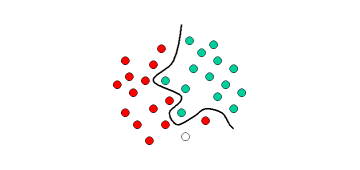
\includegraphics[scale=0.5]{images/svm1}\hspace*{-1cm}
			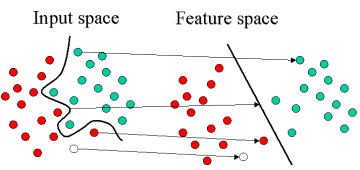
\includegraphics[scale=0.5]{images/svm2}
			\caption{Principle of support vector machines}
		\end{figure}
	\end{frame}
	\begin{frame}
		\frametitle{Gesture classification}
		\begin{figure}
			\hspace*{-1cm}
			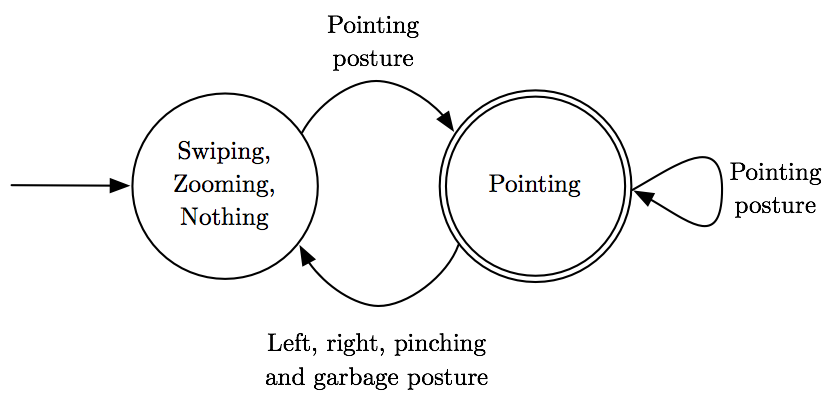
\includegraphics[scale=0.5]{images/states-pointing}
			\caption{States of pointing gesture}
		\end{figure}
			
	\end{frame}
	\begin{frame}
		\frametitle{Gesture classification}
		\begin{figure}
			\hspace*{-1cm}
			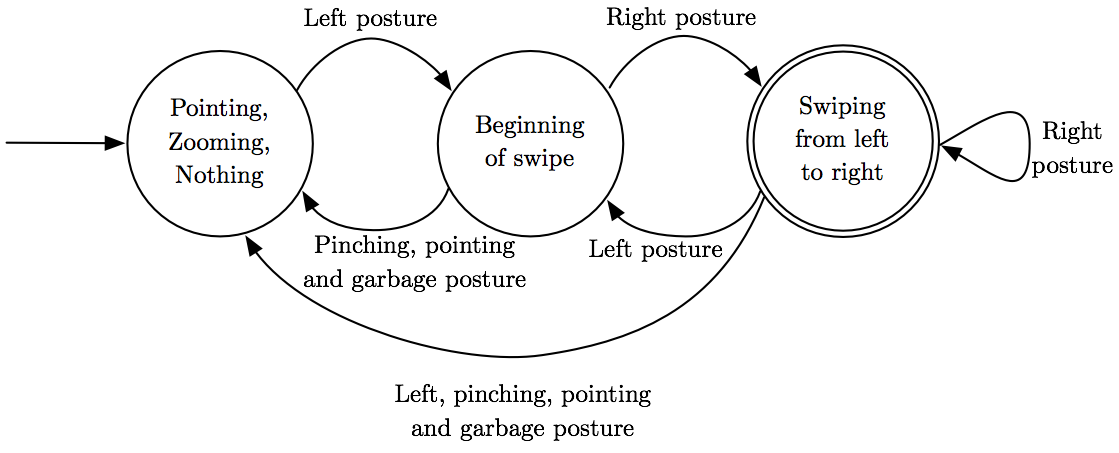
\includegraphics[scale=0.5]{images/states-swipe}
			\caption{States of swiping gesture}
		\end{figure}
	\end{frame}
	\section{Evaluation}
	\begin{frame}
		\frametitle{Evaluation}
		\begin{table}[h]
\caption{Postures and gestures of training video}
\tablestyle
\begin{tabular}{*{3}{v{1.5cm}}}
\toprule
   \tablehead gesture name &
   \tablehead number of gestures & 
   \tablehead number of postures \tabularnewline
\midrule
Nothing & 24 & 317\tabularnewline
Pointing & 5 & 397 \tabularnewline
Zooming & 6 & 253 \tabularnewline
Swiping & 12 & 78 (left) \tabularnewline
 &  & 174 (right) \tabularnewline
\bottomrule
\textbf{Total} & \textbf{47} & \textbf{1219} \tabularnewline
\bottomrule
\end{tabular}
\end{table}
	\end{frame}

\begin{frame}
		\frametitle{Evaluation}
		
\begin{table}[h]
\caption{Confusion matrix of the trained decision function}
\tablestyle
\hspace*{-2cm}
\begin{tabular}{*{6}{v{1.5cm}}}
\toprule
     &
    Garbage &
    Pointing &
    Left &
    Right &
    Zoom \tabularnewline
\midrule
\tablehead Garbage & 283 & 11 & 8 & 12 & 3  \tabularnewline
\tablehead Pointing & 14 & 383 & 0 & 0 &0  \tabularnewline
\tablehead Left & 6 & 0 & 71 & 1 & 0 \tabularnewline
\tablehead Right & 8 & 0 & 0 & 166 & 0  \tabularnewline
\tablehead Zoom & 4 & 1 & 0 & 0 & 247  \tabularnewline

\bottomrule
\end{tabular}
\label{tbl:confusion}
\end{table}
	\end{frame}
	
	\begin{frame}
		%\frametitle{Demo}
		\Huge{Demo}
	\end{frame}
	\section{Conclusion}
	\begin{frame}
		\frametitle{Conclusion}
		\begin{itemize}
			\item Gesture recognition system has fast reaction time ($<$0.4s)
			\item Gestures are easy to learn by other users
			\item Limitations: color markers have always to be seen 
			\item Gestural interfaces should rely on ergonomic features
		\end{itemize}
	\end{frame}
	\begin{frame}
		\frametitle{Future extensions}
		\begin{itemize}
			\item train more postures, investigate parametrization of SVM
			\item use HMM to classify gestures with more complex spatial and temporal dependencies
			\item replace tracking module with some other real-time capable hand-tracking system without gloves
		\end{itemize}
	\end{frame}
	\begin{frame}
		\Huge{Thank you!}
	\end{frame}
		
\end{document}
